
\section{The Audit}

\subsection{The Footnotes of Failure}

David sat across the table, the fluorescent lights above humming with the kind of corporate indifference he’d grown used to.

The regulator set the file down slowly. Flipped to the last tab.

“Are these your initials?” he asked, pointing to the bottom-right corner of a commit approval screen.

David leaned forward. Paused. Then nodded.
“Yes.”

The regulator didn’t look triumphant. Just tired.
“I spoke with the auditors this morning,” he said. “Not the first line guys — the internal forensic crew. The ones who come in after the smoke clears.”

He sat back.

“They weren’t looking to fix the system. They came to write the story. And stories need names.”

He let that land.

“They told me how it started. Not with alerts. Not with alarms. But with footprints.”

He opened the folder again, laying it flat between them.

“Timestamps. Code commits. Deployment notes. Nothing dramatic. Just… sequence. Every action left a mark.”

David stayed silent.

“They followed the trail to the model,” the regulator continued. “The one that was supposed to catch the risk. But it didn’t.”

He tapped once.

“Wrong signals. Wrong timing. Wrong assumptions for that kind of market.”

David inhaled through his nose. Said nothing.

“Then they asked how the model got out there,” the man said. “That’s where it gets… fragile.”

\begin{itemize}
\item A launch pushed two weeks early.
\item A code freeze nobody honored.
\item A patch that bypassed peer review because \textit{‘we had to move fast.’}
\end{itemize}

“And finally,” the regulator said, almost gently now, “they found the sign-off. The click that turned it all real.”

He closed the folder.

“Three letters. Lower right. Yours.”

David looked down.

There was no malice. No panic. Just a moment of quiet clarity.

Not a villain. Not even a scapegoat.

Just the name in the footnotes of failure.

\medskip

\begin{HistoricalSidebar}{Auditors vs. Regulators — Two Tribes of Postmortem Power}

  When financial systems fail, two professional species arrive: \textbf{auditors} and \textbf{regulators}. 
  Both investigate. Both ask questions. But their mandates — and temperaments — diverge in subtle, consequential ways.

  \medskip
  
  \textbf{Auditors} are internal or contracted examiners. Their job is to verify compliance with stated policies, 
  reconcile transactions, and ensure that procedures — even flawed ones — were followed. They don’t ask whether a 
  rule made sense. They ask whether it was followed and documented.

  \medskip
  
  In the 2001 Enron collapse, Arthur Andersen’s audit teams had documented procedures — but failed to challenge 
  the legitimacy of off-balance-sheet structures. They checked the math. They missed the meaning.

  \medskip
  
  \textbf{Regulators}, on the other hand, arrive on behalf of public institutions. Their mission is broader: 
  assess systemic risk, uncover governance failures, and assign accountability. While auditors scrutinize evidence, 
  regulators write the narrative. Where auditors measure, regulators interpret.

  \medskip
  
  After the 2008 crisis, agencies like the SEC, CFTC, and Financial Crisis Inquiry Commission sought more than numbers: 
  they sought names. Lehman’s liquidity “death spiral,” AIG’s collateral triggers, and Citi’s CDO masking all became 
  regulatory foci not just because rules were broken, but because stories were buried.

  \medskip
  
  In Aurora’s case, the auditors came first. They brought spreadsheets.  
  The regulators came later. They brought subtext.
  
\end{HistoricalSidebar}

\medskip

\subsection{The Room Where It Happened}

The conference room had no name — just a five-digit access code and a brass plaque that read Internal Review Suite.

Frosted glass walls blurred the outside world into abstract silhouettes. No clocks. No windows. Just the hush of recycled air and the low hum of power inside the floorboards.

David sat in the center. Not at the head of the table — there wasn’t one. The table was round. Deliberately so.

There were nine chairs.

Eight were filled.

He recognized most of them. Some by face. Some by voice. Some by reputation.

\begin{itemize}
\item The man in the tailored charcoal suit with no visible badge, who asked only short, lawyerly questions. He hadn’t introduced himself, but David knew he was Congressional counsel. The kind you didn’t interrupt.

\item Across from him, a woman in a navy skirt suit with a lanyard that bore the SEC crest — not a field agent, but someone from enforcement. Her notepad was already half full. She hadn't asked a single question yet.

\item The man beside her wore rimless glasses and carried a binder marked “Internal Risk Summary.” He hadn’t stopped flipping through it. Every highlight felt like a quiet indictment. Forensics. Probably senior.

\item On the left, near the corner, a soft-spoken man with a leather-bound legal pad and an institutional calm that made him hard to read. Office of Systemic Risk, likely. They always watched first. Always waited.

\item To David’s right, a woman he hadn’t seen in two years — formerly of Aurora Legal, now listed on internal memos as external counsel. She didn’t speak much. She didn’t need to. Her presence was message enough.

\item Then came the pair from Centauri’s audit liaison team. One was logging the session, the other just listened, watching David like he might spontaneously admit to something no one had even asked yet.

\item And finally, at the far end — an empty chair. Reserved. But for whom, David didn’t know.
\end{itemize}

\medskip

\begin{figure}[H]
  \centering
  \begin{adjustbox}{width=0.9\linewidth}
  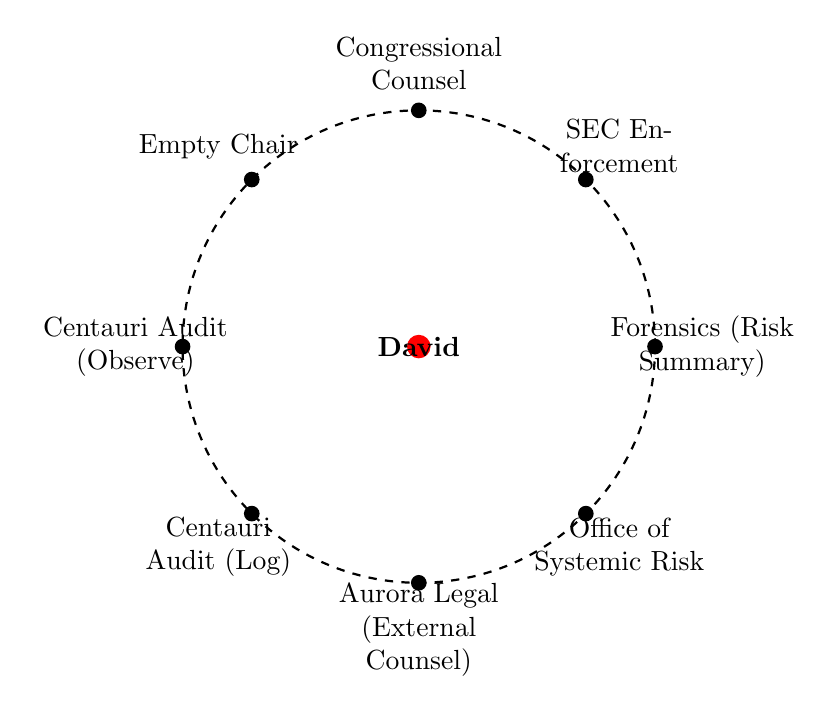
\begin{tikzpicture}
  
  % Draw circular table
  \draw[thick, dashed] (0,0) circle (3cm);
  
  % Define positions
  \foreach \angle/\name in {
      90/{Congressional Counsel},
      45/{SEC Enforcement},
      0/{Forensics (Risk Summary)},
      -45/{Office of Systemic Risk},
      -90/{Aurora Legal (External Counsel)},
      -135/{Centauri Audit (Log)},
      180/{Centauri Audit (Observe)},
      135/{Empty Chair}
  } {
      \node[circle, fill=black, inner sep=2pt] at ({3*cos(\angle)}, {3*sin(\angle)}) {};
      \node[align=center, text width=2.5cm] at ({3.6*cos(\angle)}, {3.6*sin(\angle)}) {\name};
  }
  
  % Center (David)
  \node[circle, fill=red, inner sep=3pt, label=center:{\textbf{David}}] at (0,0) {};
  
  \end{tikzpicture}
  \end{adjustbox}
  \caption{Internal Review Suite -- Seating Diagram}
\end{figure}

\medskip

The room wasn’t loud. It didn’t need to be.

There was no shouting. No drama. Just questions — methodical, unrelenting, and designed to wear a man down by inches.

David adjusted his cuff.

He wasn’t in a courtroom.

Not yet.

But the walls were thick. The doors had locks. And the floor felt like it was tilting gently underfoot — like the kind of tilt that says:
You’re not walking out of here clean.

\medskip

\begin{TechnicalSidebar}{Due Diligence, Delegation, and the Architecture of Deniability}

  David Morales believed he was protected.  
  Aurora wasn’t the contracting party. The deployment was Centauri’s. The Delaware LLC offered corporate insulation.  
  But legal shields only hold when due diligence is intact.
  
  \medskip
  
  In regulatory doctrine, \textbf{limited liability} and \textbf{role separation} are not get-out-of-jail-free cards —  
  they are privileges that assume \textit{reasonable care within one's domain}.

  \medskip
  
  Morales, as technical validator, was expected to:

  \medskip
  
  \begin{itemize}
    \item Identify and escalate model anomalies,
    \item Document suppressed signals or internal uncertainty,
    \item Ensure executive briefings were technically truthful — not just politically convenient.
  \end{itemize}

  \medskip
  
  He failed in each.  
  He didn’t lie. He didn’t conspire.  
  But he clicked “approve” on a model he knew was incomplete — and that single act converted risk into exposure.
  
  \medskip
  
  \textbf{Michael Hart}, by contrast, had engineered something else entirely:  
  \textbf{plausible deniability by design}.

  \medskip
  
  Centauri owned the deployment.  
  Aurora owned the code — but not the contract.  
  Hart held no formal role in the decision tree. He was the architect, not the executor.
  
  \medskip
  
  He didn’t need to sign anything.  
  He just needed to stage the room, whisper the timelines, and let someone else do the nodding.
  
  \medskip
  
  To a regulator, Morales was the approval trail.  
  To a court, Hart was just an advisor.  
  This was the genius of the structure: \textbf{accountability flowed downhill, but control flowed up.}
  
\end{TechnicalSidebar}

\medskip

\subsection{The Validator}

``Who approved the leverage?'' asked the Senior Forensic Analyst from the SEC, eyes steady over rimless glasses.

David sat with his hands folded, palms damp. ``The decision to raise the exposure cap came from the portfolio team. 
I wasn’t involved in that approval.''

\medskip

\begin{TechnicalSidebar}{What Is an Exposure Cap?}

  An \textbf{exposure cap} is a formal limit on the amount of financial risk that a fund, portfolio, or 
  institution is allowed to take in a specific asset class, counterparty, product type, or strategy.

  \medskip
  
  \textbf{Purpose:}

  \medskip

  \begin{itemize}
    \item To prevent over-concentration in volatile or illiquid assets.
    \item To contain downside risk during periods of stress or mispricing.
    \item To ensure regulatory or internal compliance thresholds are respected.
  \end{itemize}
  
  \medskip

  \textbf{Types of Exposure Caps:}

  \medskip

  \begin{itemize}
    \item \textit{Gross Exposure Cap:} Limits total value of positions, regardless of hedges.
    \item \textit{Net Exposure Cap:} Accounts for long vs. short positions; emphasizes directional risk.
    \item \textit{Risk-Weighted Cap:} Adjusts exposure limits based on volatility, VaR, or margin 
    requirements.
  \end{itemize}
  
  \medskip

  \textbf{Governance:}

  \medskip

  \begin{itemize}
    \item Usually set by Investment Committees or Risk Committees.
    \item Changes require formal documentation and often legal or compliance sign-off.
    \item Breaches can trigger mandatory de-risking, trading halts, or escalated reviews.
  \end{itemize}
  
  \medskip

  \textbf{Why It Matters:}  
  
  \medskip

  A raised exposure cap may unlock additional profit potential — but it also \textit{amplifies systemic 
  vulnerability}, especially if liquidity assumptions or model dependencies are flawed. When paired with 
  synthetic instruments or leveraged products, the risk scales non-linearly.
  
\end{TechnicalSidebar}

\medskip


The analyst didn’t nod. He just blinked once. ``But you provided the risk assessment, correct?''

David hesitated. ``I prepared the system output. Yes.''

``Specifically the version dated three days before the exposure increase?''

``Yes.''

The analyst flipped through a binder, stopping at a page with highlighted sections. ``According to this, the model 
flagged an increase in cross-asset volatility. Why was that column excluded in the final risk memo sent to 
Investment Oversight?''

David felt the heat rise in his neck. ``We were still calibrating the signal. At that point, it had high sensitivity 
and was generating noise—false positives.''

``And who made the decision to suppress it?''

David paused. ``Technically, I did.''

``Why?''

He swallowed. ``Because I didn’t want it to distract from the broader findings. The rest of the model showed 
acceptable thresholds.''

The analyst looked up. ``Acceptable under what assumptions?''

``Under calm regime behavior. Which, at the time—''

``—was already breaking down in commodity markets,'' the analyst interrupted gently. ``You removed the only 
indicator showing early instability. Why?''

David shifted in his seat. ``We thought it was a blip. Noise.''

``Did you note that in the report?''

``No. It didn’t seem material at the time.''

``Yet it was material enough to suppress?''

The room fell quiet.

The analyst tapped his pen once on the table. ``So, when Investment Oversight pushed the leverage increase, 
they were acting under the impression that all volatility indicators were neutral.''

David didn’t answer.

``And the one flag that wasn’t neutral — the one warning sign — was missing because you thought it might cause confusion.''

David looked down. ``I didn’t mean to mislead anyone.''

``Intent isn't the question,'' the analyst said. ``The question is whether your report enabled a decision that 
should never have been made.''

Another pause. Then:

``Mr. Morales,'' he continued, ``your name appears on the approval workflow. Not as decision-maker, but as 
validator. Your initials are here—right under the model output. Do you dispute that?''

David stared at the page.

``No,'' he said quietly. ``I don’t dispute that.''

``Thank you,'' the analyst said, and closed the binder with a soft click.

``That will do for now.''

\medskip

\begin{HistoricalSidebar}{The SEC and the Theater of Responsibility}

  Founded in the wake of the 1929 crash, the U.S. Securities and Exchange Commission (SEC) was designed as both 
  watchdog and confessor. It was designed to be part enforcement arm, and part national conscience for financial markets.

  \medskip
  
  Its mandate is simple: protect investors, ensure fair markets, and hold those accountable who threaten either. 
  But the execution is rarely so clean.

  \medskip
  
  In scenarios like David’s, the SEC doesn't storm the gates with sirens. It arrives in tailored suits and 
  calibrated language, interested less in guilt than in \textit{who signed what, and when}. It reconstructs the internal 
  machinery: approval chains, suppressed signals, reporting thresholds — all to trace how a decision came to look inevitable.

  \medskip
  
  By the time the SEC enters the room, the damage is already done. Its job is to illuminate the moment it became 
  irreversible, to identify who, and hold the flashlight on them.
  
\end{HistoricalSidebar}

\medskip

\subsection{The Signal That Wasn't Escalated}

``Why wasn’t the risk flagged?'' asked the Deputy Director of Risk Oversight from the Office of Systemic Risk.

His voice was calm, but he was already circling the failure — not of markets, but of \textit{detection}.

David took a beat. ``It depends which risk you’re referring to.''

``The synthetic credit tranche that ruptured three liquidity pools in under ninety minutes.''

\medskip

\begin{TechnicalSidebar}{What Is a Synthetic Credit Tranche?}

  A \textbf{synthetic credit tranche} is a structured financial product that slices credit exposure into 
  segments (“tranches”) based on risk level — but unlike traditional tranches, it does so using 
  \textit{derivatives}, not actual debt assets.

  \medskip
  
  \textbf{Mechanics:}

  \medskip

  \begin{itemize}
    \item Instead of holding loans or bonds, synthetic tranches use \textbf{credit default swaps (CDS)} 
    to mimic exposure.
    \item Investors in these tranches take on the risk of default in exchange for periodic premiums — 
    essentially insuring a pool of reference entities.
    \item The capital structure is divided by loss-bearing priority: equity (first-loss), mezzanine, 
    and senior tranches.
  \end{itemize}
  
  \medskip

  \textbf{Why Use Them?}

  \medskip

  \begin{itemize}
    \item Enables exposure to credit risk without directly holding the underlying assets.
    \item Offers leveraged returns for junior tranches — and perceived stability for senior ones.
    \item Appealing to funds seeking capital efficiency or directional macro exposure.
  \end{itemize}

  \medskip
  
  \textbf{Systemic Risks:}

  \medskip

  \begin{itemize}
    \item \textit{Opacity:} Synthetic tranches often lack transparency — pricing depends on internal models, 
    not market quotes.
    \item \textit{Correlation Drift:} Tranches are sensitive to correlation assumptions between entities. A 
    small shift can magnify losses dramatically.
    \item \textit{Contagion Amplifier:} Because they're derivatives, synthetic tranches create 
    \textit{counterparty exposure chains} that may ripple through the system on failure.
  \end{itemize}
  
  \medskip

  \textbf{Historical Footnote:}  

  \medskip

  Synthetic tranches played a central role in the 2008 financial crisis. Many were embedded in CDOs that assumed 
  overly optimistic default correlations — and when those assumptions broke, the losses cascaded.
  
\end{TechnicalSidebar}
 
\medskip

David exhaled slowly. ``That product was flagged — in internal simulations. We just didn’t escalate it.''

``Why not?''

``The model showed instability only in certain stress-paths. And only when run at the 95th percentile sensitivity. 
Leadership considered that noise.''

``Did you?''

David hesitated. ``I thought it needed more time. The signal hadn’t stabilized.''

``And in the meantime, the exposure increased by 31\%.''

``I wasn’t in charge of allocations.''

``No,'' the Deputy Director said. ``But your report was cited as justification in the allocation memo.''

David blinked. ``I wasn’t aware of that.''

``Page 4, footnote 2. They reference your summary of model results and cite the volatility corridor as ‘within 
tolerance.’ Was it?''

David looked down. ``Only if you exclude derivative spillover effects. Which I hadn’t tested yet.''

``So you signed off on a model summary that didn’t include derivatives — even though the product in question 
was synthetic credit?''

``We were on a compressed timeline. There was pressure to deliver a greenlight framework by end-of-quarter.''

``From whom?''

``Multiple stakeholders.''

``Can you name them?''

``I'd prefer not to speculate.''

``You don’t need to speculate, Mr. Morales. You need to remember.''

A silence stretched — not hostile, but surgical.

``Let me put it another way,'' the Deputy Director said, folding his hands. ``You were responsible for identifying 
unstable pathways in Aurora’s credit engine. And yet, the most dangerous path — the one that actually unfolded 
— wasn’t flagged, wasn’t communicated, and wasn’t contained.''

``The model wasn’t broken,'' David said quietly. ``It just wasn’t finished.''

The Director nodded slowly. ``Neither was the crisis.''

``Thank you,'' he said, closing his folder. ``That will be all for now.''

\medskip

\begin{HistoricalSidebar}{The Office of Systemic Risk --- After the Crash, the Cartographer}

  The \textbf{Office of Systemic Risk}, operating under the Financial Stability Oversight Council (FSOC), 
  was created by the Dodd–Frank Act in 2010. It is not a market regulator, but a mapmaker of collapse.

  \medskip
  
  Its mandate wasn’t to monitor firms individually, but to identify threats that emerge when interlocking 
  systems --- funds, models, margin calls, and political pressures --- align catastrophically. In other words: 
  not \textit{who} failed, but \textit{how} the system was already wired to fail.

  \medskip
  
  In cases like Aurora, the Office doesn’t arrive looking for fraud. It arrives looking for fragility that 
  was normalized — risks that were technically visible, but socially invisible. Often, the most damaging 
  decisions were made with clean hands and plausible models.

  \medskip
  
  The Office’s investigators specialize in tracing these moments: where a suppressed flag or a downgraded 
  simulation quietly mutated into systemic exposure. Their job isn’t to prevent the last crash. It’s to 
  draw the blueprint for the next one, and to ask why no one sounded the alarm when the walls were 
  already shaking.
  
\end{HistoricalSidebar}

\medskip

\subsection{Filtered Light and Governance Fog}

``Where’s the board memo?'' asked the man in the dark suit — Special Counsel for the Congressional Subcommittee 
on Financial Accountability. He spoke plainly, but each word felt like it had been cleared with legal counsel.

David looked down at the folder in front of him. ``Which memo, exactly?''

``The one documenting leadership’s awareness of the leverage adjustment and cross-product exposure. The one that 
should’ve gone to the Risk and Audit Committee in Q2. We’ve reviewed the board packets. It’s not there.''

David cleared his throat. ``If it wasn’t escalated, that would’ve been Compliance’s responsibility.''

The counsel nodded once. ``So you didn’t draft a briefing note?''

``No formal memo, no. We discussed elements of it in working groups.''

``Any minutes from those meetings?''

``Possibly. Not all sessions were minuted.''

``Were any slides presented to executive leadership?''

``There were slides,'' David said. ``But they were high-level.''

``How high-level?''

``Portfolio allocation bands. General trends. Scenario ranges.''

``Any mention of the synthetic tranche correlation drift?''

David hesitated. ``Not explicitly, no.''

The counsel glanced down at a binder. ``Your team internally referred to that drift as `uncontained contagion 
velocity’ in a Slack thread dated April 17th. Would you say that rises to the level of board visibility?''

David blinked. ``That was informal language.''

``So the board received a sanitized version?''

``They received a \textit{strategic} summary,'' David said carefully.

``Without the risks.''

``Without the emerging anomalies,'' he corrected.

``And who decided those anomalies didn’t merit inclusion?''

``That would have been a judgment call across multiple leads.''

``But your name is listed as the document owner on the draft outline. Yes?''

David didn’t answer.

The counsel didn’t press — not directly.

``Mr. Morales, when boards are kept in the dark, we investigate whether it was by accident or by design. Right now, 
it looks like your team filtered the light. That’s not a modeling issue. That’s governance.''

He closed the folder.

``And the next question will be: who gave permission... and who gave cover.''

\medskip

\begin{HistoricalSidebar}{The Congressional Subcommittee on Financial Accountability}

  The \textbf{Congressional Subcommittee on Financial Accountability} is less a financial authority and more a political 
  lens — trained on moments when markets fail and someone, somewhere, must be made to answer.

  \medskip
  
  Historically activated after high-visibility collapses --- Enron (2001), Lehman Brothers (2008), Archegos (2021) --- the 
  Subcommittee is tasked with tracing breakdowns in oversight, disclosure, and board governance. Its focus isn’t technical 
  modeling or trading algorithms; it’s \textit{who knew what, when}, and why warnings were buried, softened, or ignored.

  \medskip
  
  Unlike regulatory bodies such as the SEC or FSOC, which prioritize structural risk, the Subcommittee pursues political 
  and ethical accountability. It doesn’t ask if the system failed. It asks whether people in positions of fiduciary trust 
  failed to act.

  \medskip
  
  In hearings, terms like ``strategic ambiguity,'' ``sanitized summaries,'' and ``decision path opacity'' become signals 
  of willful negligence. In this theater, plausible deniability often reads as intent.

  \medskip
  
  The result may not be criminal indictment. Howeverr, reputational collapse begins here.
  
\end{HistoricalSidebar}




